\documentclass[10pt,a4paper]{article}
\usepackage[utf8]{inputenc}
\usepackage{amsmath}
\usepackage{amsfonts}
\usepackage{amssymb}
\usepackage{polski}
\usepackage{latexsym}
\usepackage{enumitem}
\usepackage{graphicx}

\usepackage{lastpage}
\usepackage{fancyhdr}
\pagestyle{fancy}

\fancyhf{}
\renewcommand{\headrulewidth}{0pt}
\cfoot{\thepage\ of \pageref{LastPage}}

\title{\huge AiSD - laboratorium \\ \Large Projekt zespołowy - specyfikacja funckjonalna}
\author{Kacper Baczyński, Michał Kiełczykowski, Marek Knosala, \\ Edward Sucharda}

\begin{document}

\maketitle

\section{Wstęp}

W tym dokumencie opisany został sposób korzytsania z programu, który jest celem projektu zespołowego na labolatorium przedmiotu Algorytmy i Struktury Danych prowadzonego przez Pawła Zawadzkiego w roku akademickim 2020/2021 na Wydziale Elektrycznym Politechniki Warszawskiej. Program służy do symulacji działania zespołu karetek przewożących pacjentów do szpitali. Każdy szpital ma swoją liczbę łóżek i informację ile z nich jest jeszcze wolnych. Nie zawsze szpital może przyjąć nowego pacjenta.

Szpitale mają swoje współrzędne kartezjańskie i leżą na terenie pewnego państwa. Granice tego państwa wyznacza największy wypukły wielokąt o wierzchołkach opartych na zbiorze szpitali i obiektów. Jedyna funkcjonalność obiektu to ewentualne poszerzenie granic państwa. Wybrane pary szpitali są połączone drogami, które leżą na prostej łączącej współrzędne początkowego i końcowego szpitala. Gdy dwie drogi przecinają się to jest tam skrzyżowanie. Tak więc droga z jednego szpitala do drugiego może być bezpośrednia (prosta droga z jednego punktu na mapie do drugiego) lub pośrednia, czyli taka która zawiera zmianę drogi przy przejeździe przez skrzyżowanie lub przy przejeździe przez jakiś szpital.

Gdy tylko pojawia się jakiś pacjent na terenie państwa natychmiast znajduje sie przy nim karetka i wyrusza do najbliższego szpitala w linii prostej obierając kierunek prosto na szpital, gdyż chwilowo nie musi się poruszać po drogach. Jeżeli szpital, do którego dotarła nie ma wolnych łóżek to karetka musi podróżować do kolejnego szpitala po drogach, a karetka wybiera ten szpital, do którego droga bezpośrednia lub pośrednia jest najkrótsza, podróżując tak długo aż znajdzie szpital, który może przyjąć pacjenta. Karetka nie sprawdza dwa razy tego samego szpitala. Gdy karetka odwiedza ostatni szpital i również ten nie ma wolnych łóżek, to wtedy ustawia się w kolejce do tego szpitala czekając aż się zwolni łóżko.

Poniżej znajduje się krótka specyfikacja funckjonalna, w ktorej podane zostały paramtery wejściowe, sposób uruchomienia, wygląd i działanie interfejsu graficznego oraz opis możliwych nieprawdłowych użyć i odpowiadające im komunikaty.

\section{Plik wejściowy z mapą}

Plikiem wejściowym z mapą jest plik w formacie .txt, który składa się z trzech sekcji: szpitale, obiekty oraz drogi. Sekcje są w kolejności jak podano. Każda sekcja rozpoczyna się nagłówkiem, czyli jedną linijką tekstu składającą się ze znaku ,,\#" oraz nazwy sekcji. W dalszej części sekcji są wiersze z danymi dotyczące danej sekcji.

Każda z sekcji ma swój unikalny porządek danych. W przypadku szpitali każdy wiersz składa się z:
\begin{itemize}
\item identyfikatora szpitala, które musi być unikalną, nieujemną liczbą całkowitą
\item nazwy szpitala, która jest dowolnym ciągiem znaków za wyjątkiem znaku ,,$\mid$"
\item współrzędenj w osi \textit{x}, która oznacza położenie w tej osi danego szpitala, która musi być liczbą całkowitą
\item współrzędenj w osi \textit{y}, która oznacza położenie w tej osi danego szpitala, która musi być liczbą całkowitą
\item liczby łóżek w szpitalu, która musi być liczbą dodatnią całkowitą
\item liczby wolnych łóżek w szpitalu, która musi być liczbą nieujemną całkowitą i mniejszą od liczy łóżek w szpitalu
\end{itemize}
W przypadku obiektów każdy wiersz składa się z:
\begin{itemize}
\item identyfikatora obiektu, który musi być unikalną, nieujemną liczbą całkowitą
\item nazwy obiektu, która jest dowolnym ciągiem znaków za wyjątkiem znaku ,,$\mid$"
\item współrzędenj w osi \textit{x}, która oznacza położenie w tej osi danego obiektu, która musi być liczbą całkowitą
\item współrzędenj w osi \textit{y}, która oznacza położenie w tej osi danego obiektu, która musi być liczbą całkowitą
\end{itemize}
W przypadku połączeń dróg każdy wiersz składa się z:
\begin{itemize}
\item identyfikatora drogi, który musi być unikalną, nieujemną liczbą całkowitą
\item identyfikatora jednego szpitala, który musi być poprzednio zdefiniowany
\item identyfikatora drugiego (innego) szpitala, który musi być poprzednio zdefiniowany
\item odległości między szpitalami z poprzednich dwóch punktów, która musi być liczbą całkowitą, dodatnią
\end{itemize}

Każde wyrażenie w linijce każdej sekcji jest oddzielone od kolejnego dowolną liczbą spacji przed i po dokładnie jednym znaku ,,$\mid$". Po ostanim wyrażeniu jak i przed pierwszym nie ma znaku ,,$\mid$", ale może być dowolnie dużo spacji. W pliku niedozwolone są puste linie. Sekcja szpitali musi zawierać dane z przynajmniej jednym wierszem. Nie może istnieć więcej niż jedna bezpośrednia droga ze jednego do drugiego szpitala.

Przykładowy plik wejściowy z mapą umieszczono poniżej:
\begin{description}[style=multiline,leftmargin=3cm]
\item \# Szpitale
\item 1 $\mid$ Szpital Wojewódzki nr 997 $\mid$ 10 $\mid$ 10 $\mid$ 1000 $\mid$ 100
\item 2 $\mid$ Krakowski Szpital Kliniczny $\mid$ 100 $\mid$ 120 $\mid$ 999 $\mid$ 99
\item 3 $\mid$ Pierwszy Szpital im. Prezesa RP $\mid$ 120 $\mid$ 130 $\mid$ 99 $\mid$ 0
\item 4 $\mid$ Drugi Szpital im. Naczelnika RP $\mid$ 10 $\mid$ 140 $\mid$ 70 $\mid$ 1
\item 5 $\mid$ Trzeci Szpital im. Króla RP $\mid$ 140 $\mid$ 10 $\mid$ 996 $\mid$ 0
\item \# Obiekty 
\item 1 $\mid$ Pomnik Wikipedii $\mid$ -1 $\mid$ 50
\item 2 $\mid$ Pomnik Fryderyka Chopina $\mid$ 110 $\mid$ 55
\item 3 $\mid$ Pomnik Anonimowego Przechodnia $\mid$ 40 $\mid$ 70
\item \# Drogi
\item 1 $\mid$ 1 $\mid$ 2 $\mid$ 700
\item 2 $\mid$ 1 $\mid$ 4 $\mid$ 550
\item 3 $\mid$ 1 $\mid$ 5 $\mid$ 800
\item 4 $\mid$ 2 $\mid$ 3 $\mid$ 300
\item 5 $\mid$ 2 $\mid$ 4 $\mid$ 550
\item 6 $\mid$ 3 $\mid$ 5 $\mid$ 600
\item 7 $\mid$ 4 $\mid$ 5 $\mid$ 750
\end{description}

\section{Plik wejściowy z pacjentami}

Plik wejściowy z pacjentami musi być w formacie .txt i składać się z jedego nagłówka i jednej sekcji. Nagłówek ma strukturę jak w pliku wejściowym z mapą. Sekcja natomiast na składa się z uporzątkowanych wierszy według następującej kolejności:
\begin{itemize}
\item identyfikatora pacjenta, który musi być unikalną, nieujemną liczbą całkowitą
\item współrzędenj w osi \textit{x}, która oznacza położenie w tej osi danego pacjenta, która musi być liczbą całkowitą
\item współrzędenj w osi \textit{y}, która oznacza położenie w tej osi danego pacjenta, która musi być liczbą całkowitą
\end{itemize}
Przykładowy plik wygląda następująco:
\begin{description}[style=multiline,leftmargin=3cm]
\item \# Pacjenci
\item 1 $\mid$ 20 $\mid$ 20
\item 2 $\mid$ 99 $\mid$ 105
\item 3 $\mid$ 23 $\mid$ 40
\end{description}

\section{Uruchomienie programu}

Program można uruchomić z terminala. Aby to zrobić trzeba zainstalować na komputerze środowisko uruchomieniowe JRE języka Java. Gdy ten wymóg jest już spełniony należy w lokalizacji pliku ProjektZespolowy.jar otworzyć temrminal i wpisać komendę: \\
\\
\textsl{java -jar ProjektZespolowy.jar}

\section{Interfejs Graficzny}

Po porawnym uruchomieniu programu pokazuje się okno intersejsku graficznego. Wygląd takiego okna widać na Rysunku nr 1.

\begin{figure}[h]
  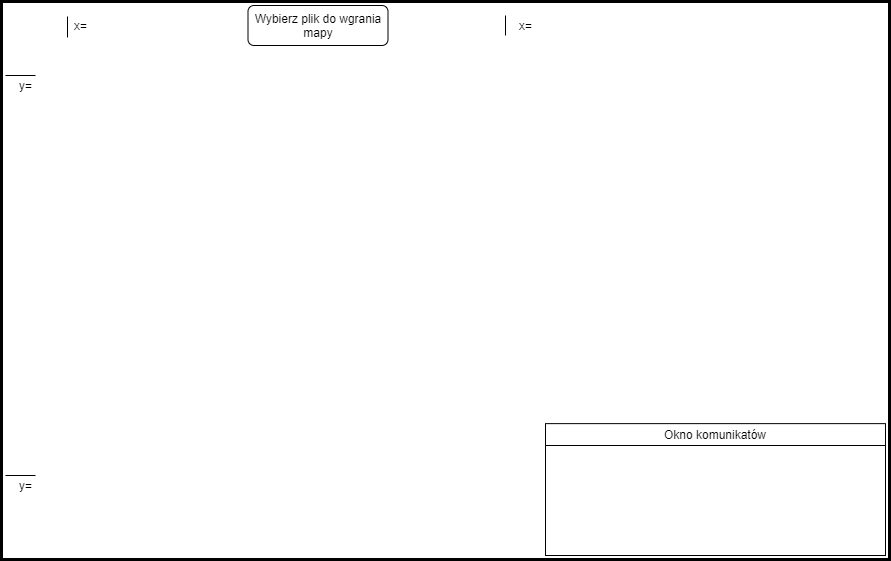
\includegraphics[width=\linewidth]{./images/startowy_widok.png}
  \caption{Widok startowy.}
  \label{fig:GUIstart}
\end{figure}

W prawym dolnym rogu znajduje się okno komunikatów. W górnej części znajduje sie przycisk ,,wybierz plik do wgrania mapy", który należy wciskąć aby wybrać z komputera plik wejściowy z mapą. Dodatkowo widoczne są 4 krótkie odcinki. Dwa pionowe będą oznaczyły skrajne wartości punktów zaznaczonych na mapie w osi \textit{x} a obok nich pojawią się odpowiadające im wartości. Analogicznie odcinki poziome oznaczają skrajne wartości punktów zaznaczonych na mapie w osi \textit{y} a obok nich odpowiadające im wartości. Po wgraniu poprawnego pliku pojawia się mapa państwa i dodatkowe przyciski jak na Rysnuku 2.

\begin{figure}[h]
  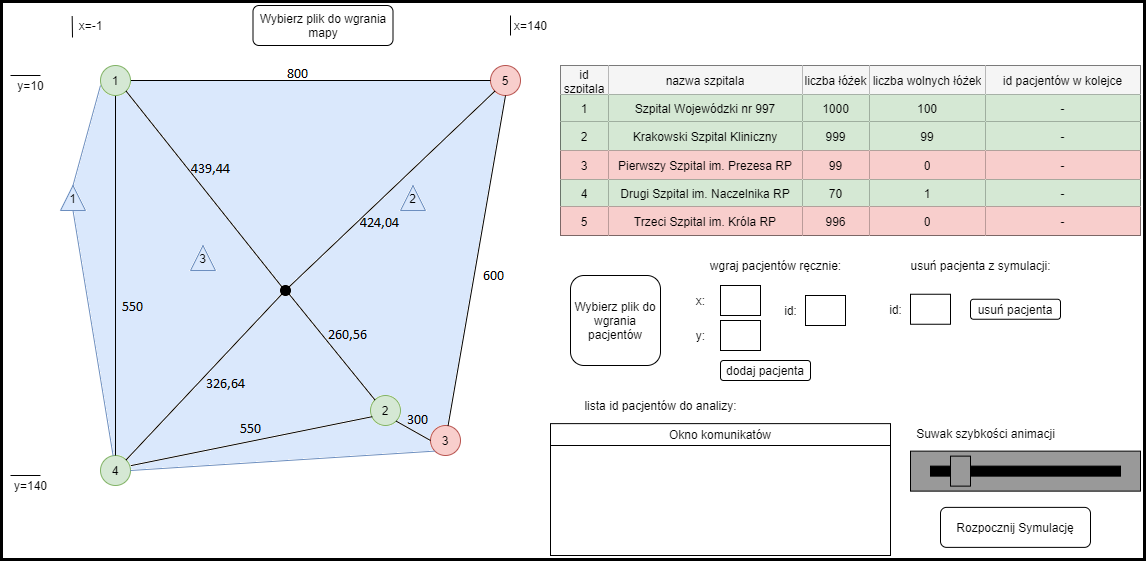
\includegraphics[width=\linewidth]{./images/widok_z_mapa.png}
  \caption{Widok po załadowaniu mapy.}
  \label{fig:GUImap}
\end{figure}

Terytorium państwa ma niebieskie tło. Obiekty oznaczono kształtem trójkąta wewnątrz którego znajduje się jego identyfikator, który zostało podany w pliku wejściowym. Kołami oznaczono szpitale. Jeśli w danym szpitalu są jeszcze miejsca to jest to koło koloru zielonego w przeciwnym przypadku koło koloru czerwonego. Wewnąrz koła znajduje się identyfikator zgodny z plikiem wejściowym. Odcinki koloru czarnego na mapie to drogi. Droga na mapie ma początek i koniec w szpitalu lub na skrzyżowaniu. Zatem niektóre drogi z pliku wejśiowego z mapą zostały podzielone na mniejsze z uwagi na skrzyżowania. W okolicy środka każdej drogi została podana wartość jej długości. Czarną kropką zostały oznaczone na mapie skrzyżowania. Po wgraniu mapy pojawiły się skrajne wartości występujące na mapie przy odcinkach, które były już widoczne przed załadowaniem mapy.

Po prawej stronie od mapy na samej górze znajduje się tabela, która zawiera rekordy szpitali: ich identyfikator, nazwę, liczbę łóżek, liczbę wolnych łóżek i kolejkę pacjentów oczekujących na przyjęcie do danego szpitala. Kolejka składa się z ciągu identyfikatorów pacjentów oddzielonych przecinkami. Jeżeli dany szpital nie ma wolnych łóżek wiersz jest w kolorze czerwonym. W przeciwnym przypadku jest koloru zielonego.

Poniżej tabeli z informacjami o szpitalach znajdują się 3 sekcje operacji na pacjentach. Pierwszy obiekt z lewej to przycisk o nazwie ,,Wybierz plik do wgrania pacjentów", który służy do wgrywania pliku wejściowego z pacjentami. Druga sekcja składa się z trzech pól do wpisywania liczb oraz przycisku do dodwawania pacjentów. Aby dodać pacjenta użytkownik musi podać jego współrzędne \textit{x}, \textit{y} oraz jego identyfikator, a następnie wcisnąć przycisk ,,dodaj pacjenta". Trzecia sekcja służy do usuwania pacjentów, których użytkownik nie będzie chciał poddawać symulacji, a już dodał go za pomocą jednej z poprzednich dwóch sekcji. Dla wybranego pacjenta należy wpisać jego identyfikator w pole do wpisywania liczb oraz wcisnąć przycisk ,,usuń pacjenta". Lista identyfikatorów pacjentów, którzy będą podani symulacji po jej uruchomieniu znajduje się nad oknem komunikatów. Kojene identyfikatory są oddzielane przecinkami, a kolejność jest zgodna z kolejnością wprowadzania kolejnych pacjentów.

Na prawo od okna komunikatów znajudje się przycisk ,,Rozpocznij Symylację", który blokuje wprowadznie nowych pacjentów oraz zmianę mapy i dokonuje animacji transportowania pacjentów do szpitala w kolejności jak zostali wprowadzani do programu. Nad przyciskiem ,,Rozpocznij Symulację" znajduje się suwak regulujący szybkość animacji.

\section{Przebieg animacji}

Po wciśnięciu przycisku ,,Rozpocznij Symulację" na mapie pokazują wszyscy pacjenci jako pomarańczowe kropki. Następnie każda kropka oznaczająca pacjenta, według kolejności na liście pacjentów poddawanych symulacji, zaczyna się przemieszczać. Dodatkowo zostawia za sobą łamaną w postaci przebytej trasy w kolorze pomarańczowym. Widok takiego przemieszczania się pacjenta oraz pozostałych pacjentów czekających na swoją kolej został pokazany na Rysnuku 3.

\begin{figure}[h]
  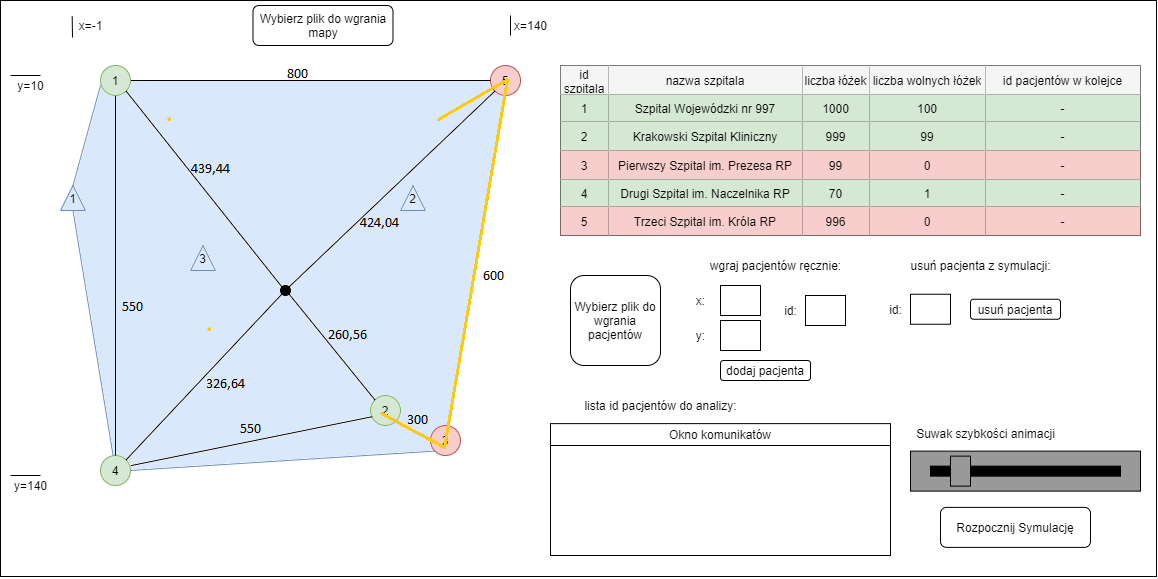
\includegraphics[width=\linewidth]{./images/widok_symulacji.png}
  \caption{Widok symulacji.}
  \label{fig:GUIsym}
\end{figure}

Gdy dany punkt dotrze do szpitala gdzie jest wolne miejsce pojawia się stosowny komunikat informujący o przyjęciu pacjenta o danym identyfikatorze do szpitala o danym identyfikatorze. Następuje aktualizacja liczby wolnych miejsc w danym szpitalu i ewentualnie zmiana jego koloru na mapie i w tabeli na kolor czerwony. Następnie znika punkt symbolizujący dopiero co przyjętego pacjęta z mapy jak róznież znika jego trasa. Dalej jest inicjalizowane rozpoczęcie animacji trasy kolejnych pajentów. Jeżeli dla danego pacjenta nie starczy miejsca w żadnym szpitalu, do którego może dojechać karetka, to pojawia się o tym komunikat w oknie komunikatów. Napstępnie identyfikator tego pacjenta jest dodawany w tabeli szpiatali do listy identyfikatorów pacjentów w kolejce. Następnie znika punkt i jego trasa a rozpoczyna sie symulacja kolejnego pacjenta. Jeżeli jakiś pacjent jest poza granicami państwa to pojawia się o tym komunikat. Następnie znika on z mapy i następuje animacja kolejnego pacjenta. Gdy już wszysycy pacjenci zostali poddani symulacji w oknie komunikatów pojawia sie komunikat o zakończeniu symulacji. Program dalej ma zapisane w pamięci mapę i pacjetnów, więc można dowolnie wiele razy wykonywać symulację. Aby zakończyć działanie programu należy wycisnąć przycisk ESC.

\section{Możliwe komunikaty w oknie komunikatów}
Poniżej przedstawiono listę komunikatów, które mogą pojawić się w oknie komunikatów. Są to komunikaty zrówno o poprawnie wykonanych operacjach przez program jak i komunikaty o błędnym użyciu programu przez użytkownika. Komunikaty o błędzie:
\begin{itemize}
\item początek pliku nie rozpoczyna się od znaku \#: \\ \textbf{Błąd: początek pliku nie rozpoczyna się od znaku \#}
\item pusty plik: \\ \textbf{Błąd: wgrywany plik jest pusty}
\item brak nawet jednego rekordu w sekcji szpitali: \\ \textbf{Błąd w linii \textless numer linii\textgreater: brak rekorów w sekcji szpitali}
\item zbyt dużo znaków ,,$\mid$" w linii: \\ \textbf{Błąd w linii \textless numer linii\textgreater: zbyt dużo znaków ,,$\mid$"}
\item zbyt mało znaków ,,$\mid$" w linii: \\ \textbf{Błąd w linii  \textless numer linii\textgreater: za mało znaków ,,$\mid$"}
\item niezgodny typ danych: \\ \textbf{Błąd w linii  \textless numer linii\textgreater: niezgodny typ danych}
\item liczba jest ujemna gdy wymagana jest nieujemna: \\ \textbf{Błąd w linii  \textless numer linii\textgreater: podana wartość nie może być ujemna}
\item liczba jest niedodatnia, gdy wymagana jest dodatnia: \\ \textbf{Błąd w linii \textless numer linii\textgreater: podana wartość musi być dodatnia}
\item identyfikator szpitali, obiektów lub dróg nie jest unikalny: \\ \textbf{Błąd w linii  \textless numer linii\textgreater : identyfikator tego Szpitala/Obiektu/Drogi został już przypisany do innego Szpitala/Obiektu/Drogi}
\item w połączeniach jest użyty identyfikator szpitala, który nie istnieje: \\ \textbf{Błąd w linii  \textless numer linii\textgreater: brak szpitala o podanym identyfikatorze}
\item redefinicja drogi: \\ \textbf{Błąd w linii \textless numer linii\textgreater : połączenie między podanymi dorgami zostało już zdefiniowane}
\end{itemize}

Gdy plik wejściowy jest prawidłowy i program zaczyna działać prawidłowo, możliwe są następujące komunikaty:
\begin{itemize}
\item poprawnie wczytano mapę:\\ \textbf{Info: Mapa załadowna.}
\item poprawnie wczytano listę pacjentów:\\ \textbf{Info: Lista pacjentów załadowana.}
\item rozpoczęcie animacji kolejnego pacjenta:\\ \textbf{Info: Rozpoczpoczęcie ratowania pacjenta nr \textless identyfikator pacjenta\textgreater} 
\item pacjent został przyjęty do szpitala:\\ \textbf{Info: pacjent został przyjęty do szpitala nr \textless identyfikator szpitala\textgreater}
\item pacjent nie znalazł miejsca w tym szpitalu i przemieszcza się do następnego:\\ \textbf{Info: pacjent nie znalazł miejsca w tym szpitalu nr \textless identyfikator szpitala\textgreater}
\item pacjent nie znalazł miejsca w żadnym szpitalu, więc ustawia się w kolejce do ostatniego szpitala, do którego dotarł\\ 			\textbf{Info: pacjent czeka w kolejce do szpitala nr \textless identyfikator szpitala\textgreater}
\item pacjent poza granicami państwa: \\ \textbf{Info: pacjent poza granicami państwa. Brak działań ratunkowych.}
\item koniec symulacji \\ \textbf{Info: Koniec symulacji.}
\end{itemize}

\section{Źródła}
Wykorzystane przykłady pliku wejściowego z mapą i pliku wejścowego z pacjentami są stworzone przez Pawła Zawadzkiego z Wydziału Elektrycznego Politechniki Warszawskiej w 2020 roku.

\end{document}{article}


